

\documentclass[twocolumn,10pt]{article}

\usepackage[utf8]{inputenc}

 \usepackage[T1]{fontenc}
\usepackage{xcolor}
\usepackage{float}
\usepackage{graphicx}
\usepackage{siunitx}
\usepackage{geometry}
\usepackage{float}
\usepackage[toc,page]{appendix}
\graphicspath{ {./figuren/} }
\usepackage{fancyvrb}
\usepackage{hyperref}
\hypersetup{
    colorlinks = true,
    linkcolor = blue,
    citecolor=blue,
    linkbordercolor = {white},
}
\usepackage{fullpage}
\usepackage{fancyvrb}
\graphicspath{ {./figuren/} }

\geometry{
    a4paper,
    left=20mm,
    right=20mm,
    top=25mm,
    bottom=25mm,
}

\frenchspacing
\usepackage{booktabs}
\usepackage{microtype}

\usepackage[english,dutch]{babel}

\usepackage{listings}
\lstset{
    belowcaptionskip=1\baselineskip,
    breaklines=true,
    columns=flexible,
    basicstyle=\small\ttfamily,
}
\usepackage{graphicx}
\usepackage{placeins}

\usepackage{xcolor}
\usepackage{titlesec}
\titleformat{\section}[block]{\color{blue}\Large\bfseries\filcenter}{}{1em}{}
\titleformat{\subsection}[hang]{\bfseries\filcenter}{}{1em}{}

\usepackage{mathtools}

\title{Opdracht 2, Algoritmiek}
\author{Jenny Vermeltfoort, s3787494, groep PO2\_20}

\begin{document}

\selectlanguage{dutch}
\def\tablename{Tabel}

\maketitle

\section*{Uitleg}
Cryptarithm is een puzzel waarbij er waardes worden toegekend aan de letters van drie verschillende woorden. Het doel is om een unieke waarde toe te kennen aan elke unieke letter zodat de som van de eerste twee woorden leidt tot het cijfer voorgekomen uit de waardes van het derde woord. Er mogen in deze oplossing geen leading nullen staan. 

Dit document beschrijft de implementatie van een backtracking algoritme om cryptarithmische puzeels op te lossen. De implementatie kan ook bepalen hoeveel unieke puzzels (puzzels met maar 
\'e\'en oplossing) er geconstrueerd kunnen worden met twee woorden.


\section*{Zoek oplossing}
Om zoek\_oplossing voor te bereiden worden er letters uit alle woorden gehaald op de volgorde zoals beschreven in de figuur hieronder. Voor elke letter wordt bijgehouden in welke kolom de letter voor het eerst voorkomt. 

In de zoek\_oplossing implementatie wordt de p->letters[] lijst op volgorde toegekend. De puzzel wordt per kolom ($K0.. K_n$) geverifieerd. Dit wordt gedaan met een achterlopende kolom index. Wanneer bijvoorbeeld de letter 'O' wordt toegekend uit het voorbeeld hieronder zal kolom K0 worden geverifieerd. Dit wordt gedaan door de waarde van E te berekenen, alle waardes hiervoor zijn bekend ($\text{waarde letter woord0} + \text{waarde letter woord1} + \text{carry}_{K0}$). Deze waarde moet niet al toegekend zijn aan een andere letter, en als de letter E al is toegekend dan moet de toegekende waarde hetzelfde zijn als de waarde die is berekend met de waardes uit de kolom. Is dit niet het geval gaat de implementatie een stapje terug. Bij letter 'B' in het voorbeeld worden de kolommen K1 en K2 geverifieerd op dezelfde manier als hierboven voordat B wordt toegekend.

De linkse letter van het het laatste woord kan al bepaald worden wanneer de lengte van dit woord groter is als beide voorgaande woorden. Deze waarde is namelijk 1 en de carry van deze kolom is ook 1.

Wanneer alle waardes zijn toegekend wordt gecontroleerd of er geen leading nullen zijn en of de carry van de laatste kolom niet 0 of 1 is afhankelijk van het lengte verschil van woord2 en woord0/woord1.

Oorspronkelijk had ik een implementatie gemaakt waarbij alle kolommen waar een reeds toegekende letter in zit werden gecontroleerd. Hiervoor werd per kolom gekeken of er genoeg informatie bekend was om de bepalen of de puzzel nog een oplossing heeft (De carry$_{K(n+1)}$ kon al bepaald zijn bijvoorbeeld, hierdoor moeten de waardes van $K_n$ minimaal samen groter dan het grondgetal zijn. Of heel simpel voor alle toegekende kolommen de som van het derde woord berekenen en kijken of dit nog beschikbaar is.) Hierdoor werd de tijdcomplexiteit minder, echter werdt de logica per iteratie aanzienlijk cpu-cycle zwaar (veel branching en weining ruimtelijke localiteit voor caching, daarbij een hogere cache miss rate) wat leidde tot langere iteratie tijden. Er was hier waarschijnlijk nog wel wat optimalisatie te winnen, echter ben ik persoonlijk tevreden met de huidige implementatie.

\begin{figure}[H]
    \centering
    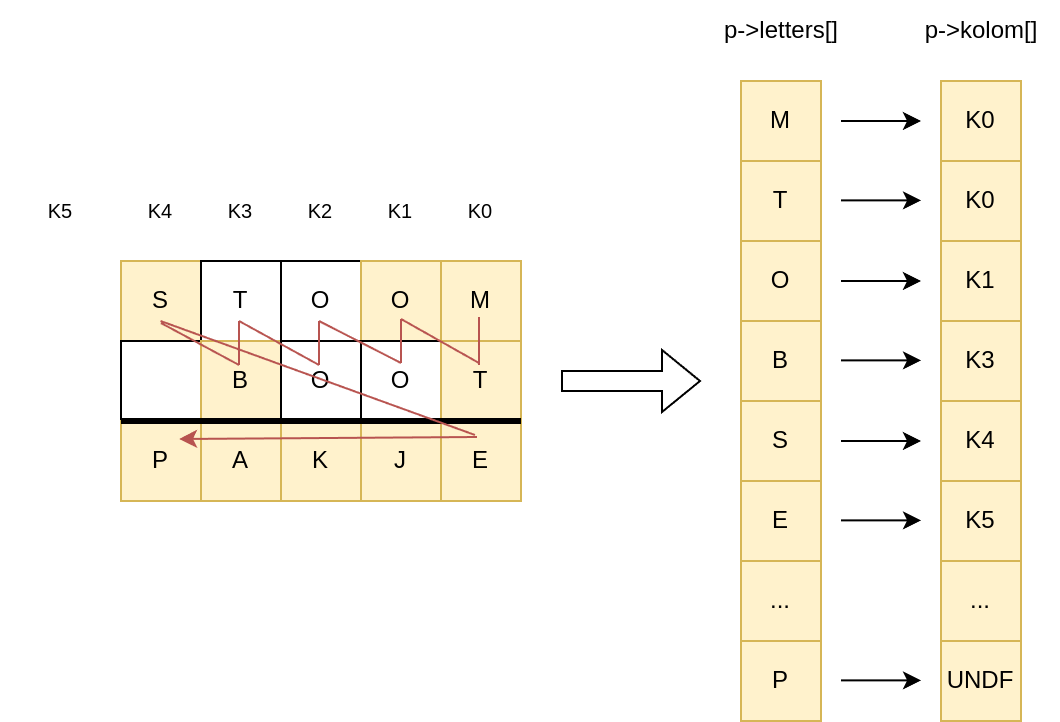
\includegraphics[width=1.0\columnwidth]{letter.png}
        \caption{Sorteer orde.}
    \end{figure}
    \hfill


\subsection*{Oplossingen}
Voor een puzzel $A+B=B$ en $\text{grondgetal} >= 2$ bestaan er grondgetal $- 1$ hoeveelheid oplossingen. Dit komt omdat $A=B-B=0$ waardoor er voor B grondgetal $- 1$ aantal keuzes zijn. Hierbij is er wel vanuit uitgegaan dat leading nullen toegestaan zijn.

Voor de puzzel $A+B=CD$, grondgetal 10 en $A < B$ bestaan er 15 oplossingen, dit komt doordat $C=1$ aangezien het maximale van CD $9+9=18$ is en er mogen geen leading nullen bestaan, dus $CD >= 10$. Dit betekend dat $A+B >= 10$, en dus $6 <= B <= 9$ aangezien $A < B$. De hoeveelheid opties voor $A$ is niet bepaald wiskundig te omschrijven, $A$ mag in ieder geval geen 1 of 0 zijn en heeft de constrain dat $A >= 10 - B$. Daarom voor elke B betekend dit:
\begin{table}[h]
    \centering
    \caption{Beredenering $A$.}
        \begin{tabular}{@{}ccc@{}}
            \toprule
            B & Opties A & Aantal \\ 
            \midrule
            6 & $\{4\}$ & 1 \\
            7 & $\{3, 5, 6\}$ & 3 \\
            8 & $\{2, 4, 5, 6, 7\}$ & 5 \\
            9 & $\{3, 4, 5, 6, 7, 8\}$ & 6 \\
            \bottomrule
        \end{tabular}
\end{table}
\FloatBarrier
Het totaal aantal oplossingen, zonder de eis $A<B$ is dus de bovengenoemde beredenering maal twee, dus 30 oplossingen.


\begin{table}[h]
    \centering
    \caption{Resultaten van verschillende puzzels.}
    \resizebox{1.0\columnwidth}{!}{ 
        \begin{tabular}{|p{0.10\textwidth}|p{0.03\textwidth}|p{0.05\textwidth}|p{0.065\textwidth}|p{0.06\textwidth}|}
            \hline
            Puzzel & G.g. & Opl. & Bekeken & Tijd \\ 
            \hline
            STOOM + BOOT = PAKJE & 10 & 5      & 1099 & \SI{29}{\micro\second} \\
            \hline
             & 9 & -1       & 229 & \SI{5}{\micro\second} \\
            SINT + & 10 & 16      & 397 & \SI{14}{\micro\second} \\
            PIET = & 11 & 64      & 859 & \SI{21}{\micro\second} \\
            RUZIE & 20 & 11068   & 40482 & \SI{883}{\micro\second} \\
            & 26 & 53590   & 162415 & \SI{3264}{\micro\second} \\
            \hline
            N=3, P=21 & 26 & 213 & 733  & \SI{13}{\micro\second} \\
            \hline
        \end{tabular}
    }
\end{table}
\FloatBarrier

\section*{Construeer puzzel}
Wanneer een puzzel wordt geconstrueerd uit twee woorden zijn er letters waarbij de waarde afhankelijk is van de twee woorden. Dit zijn alle unieke letters van deze twee woorden, daarom moet voor elke positie van het laatste woord de 'onvrije' letters getest worden. Er bestaat ook een set van vrije letters, dit zijn alle letters die niet in de twee woorden staan, maar die genoodzaakt zijn te bestaan omdat er een grondgetal hoeveelheid aan unieke letters kan bestaan.

Een voorbeeld: voor de puzzel SINT+PIET=... voor grondgetal 10 is de set onvrije letters: $\{\underbar{S}, \underbar{I}, \underbar{N}, \underbar{T}, \underbar{P}, \underbar{E}\} \subseteq S_o$ en de set van vrije letters: $\{ \underbar{A}, \underbar{B}, \underbar{C}, \underbar{D} \} \subseteq S_v$. De implementatie maakt de lijst van vrije letters van A tot Z waar de letter niet in \'e\'en van de twee woorden bestaat.

Om ervoor te zorgen dat elke oplossing uniek is, worden er opbouwend meer vrije letters gekozen naarmaten de opbouw van het laatste woord vorderd. Het laatste woord word van links naar rechts opgebouwd. Er is een limiet gesteld per positie op de hoeveelheid vrije letters die er gekozen kunnen worden. Beginnende met een limiet van 1. Wanneer er een vrije letter wordt gekozen in een linkse positie dan heeft de volgende positie keuze uit een vrije letter meer, dit proces volgt voor alle opeenvolgende posities totdat alle vrije letters gekozen kunnen worden.

Een voorbeeld, met de twee sets gedifineer hierboven: wanneer voor positie 1 (de meest linker positie) de vrije letter A is gekozen, dan heeft positie 2 keuze uit $S_o \cup \{\underbar{A}, \underbar{B}\}$ en wanneer voor positie 2 de vrije letter B is gekozen heeft de positie 3 keuze uit: $S_o \cup \{\underbar{A}, \underbar{B}, \underbar{C}\}$. Dus wanneer op positie 2 een letter uit $S_o$ wordt gekozen blijft de keuze voor de volgende positie $S_o \cup \{\underbar{A}, \underbar{B}\}$. Door deze methode is de structuur van de vrije letters uniek en zal bijvoorbeeld AAB worden geconstrueerd, maar BBA niet.

Zie de tabel hieronder voor de resultaten van verschillende puzzel constructies.
\begin{table}[h]
    \centering
    \caption{Resultaten van verschillende constructies.}
    \resizebox{\columnwidth}{!}{ % Verklein de tabel naar de kolombreedte
        \begin{tabular}{|p{0.2\textwidth}|p{0.05\textwidth}|p{0.07\textwidth}|p{0.08\textwidth}|}
            \hline
            Woorden & G.g. & Puzzels & Tijd \\ 
            \hline
            SINT + PIET = ... & 10 & 752 & \SI{0.088}{\second} \\
            \hline
            KLAAS + PAARD = ... & 10 & 20692 & \SI{4.386}{\second} \\
            \hline
            MIJTER + MANTEL = ... & 10 & 550024 & \SI{120.247}{\second} \\
            \hline
        \end{tabular}
    }
\end{table}
\FloatBarrier

\section*{Heuristiek}
Voor puzzel $SINT+KLAAS=...$ bij grondgetal 9 worden er 5489 unieke puzzels gevonde.
Om de heuristiek van mijn code te verifieren heb ik een aantal testen uitgevoerd op deze puzzel.
Het volgende is gecontroleerd:
\begin{itemize}
    \item Alle gevonden puzzels zijn daadwerkelijk uniek. (A+B=C en B+A=C) zijn uniek.
    \item Gecontroleerd of alle puzzels daadwerkelijk maar 1 oplossing hebben met een brute force algoritme.
    \item Gecontroleerd of alle puzzels correct zijn met een externe base 9 calculator, dus (A+B=C) in base 9.
\end{itemize}

\begin{lstlisting}
    $ rm SINT_KLAAS_oplossingen.txt ; for t in $(cat SINT_KLAAS_gevonden_puzzels.txt) ; do echo "1 9 SINT KLAAS $t 3 4 3" | ./WoordSomPuzzel >> SINT_KLAAS_oplossingen.txt ; done
    $ cat SINT_KLAAS_oplossingen.txt | grep "De puzzel kent" | grep -v "De puzzel kent 1" # kijk of er puzzels met meer dan 1 oplossingen zijn.
    $ cat SINT_KLAAS_oplossingen.txt | grep "^ T=. S=" | sort | uniq -c | awk '$1 > 1' # kijk of alle letter allocaties uniek zijn.
    $ cat SINT_KLAAS_alle_sommen_met_flip.txt | sort | uniq -c | awk '$1 > 1' # kijk of sommen, dus alle puzzels uniek zijn.
    $ cat SINT_KLAAS_brute_force.txt | grep "De puzzel kent" | awk '$4 > 1' $ kijk of alle puzzels maar 1 unieke oplossing kennen.
    $ ./valideer_alle_sommen.sh # controleert of alle sommen in SINT_KLAAS_alle_sommen_met_flip.txt goed zijn.
\end{lstlisting}


\newpage
\begin{appendices}
    \section*{Experimenten Logs}
    \begin{lstlisting}

        De puzzel kent 5 verschillende oplossing(en).
        Het zoeken van de oplossingen kostte 28 clock ticks, ofwel 2.8e-05 seconden.
        We hebben daarbij 1099 deeloplossingen bekeken.
        Een gevonden oplossing is:
        M=2 T=7 O=5 B=8 S=3 E=9 J=0 K=1 A=6 P=4
        Grondgetal: 10 
        Puzzel:
        0: STOOM
        1: BOOT
        2: PAKJE
        Toegekende letters:

        De puzzel kent -1 verschillende oplossing(en).
        Het zoeken van de oplossingen kostte 5 clock ticks, ofwel 5e-06 seconden.
        We hebben daarbij 229 deeloplossingen bekeken.
        Grondgetal: 9 
        Puzzel:
        0: SINT
        1: PIET
        2: RUZIE
        Toegekende letters:
        R=1; 

        De puzzel kent 16 verschillende oplossing(en).
        Het zoeken van de oplossingen kostte 14 clock ticks, ofwel 1.4e-05 seconden.
        We hebben daarbij 397 deeloplossingen bekeken.
        Een gevonden oplossing is:
        T=2 N=5 E=4 I=9 S=6 P=3 Z=8 U=0 R=1
        Grondgetal: 10 
        Puzzel:
        0: SINT
        1: PIET
        2: RUZIE
        Toegekende letters:
        R=1; 

        De puzzel kent 64 verschillende oplossing(en).
        Het zoeken van de oplossingen kostte 21 clock ticks, ofwel 2.1e-05 seconden.
        We hebben daarbij 859 deeloplossingen bekeken.
        Een gevonden oplossing is:
        T=2 N=6 E=4 I=10 S=7 P=8 Z=9 U=5 R=1
        Grondgetal: 11 
        Puzzel:
        0: SINT
        1: PIET
        2: RUZIE
        Toegekende letters:
        R=1; 

        De puzzel kent 11068 verschillende oplossing(en).
        Het zoeken van de oplossingen kostte 883 clock ticks, ofwel 0.000883 seconden.
        We hebben daarbij 40482 deeloplossingen bekeken.
        Een gevonden oplossing is:
        T=2 N=3 E=4 I=7 S=5 P=15 Z=14 U=0 R=1
        Grondgetal: 20 
        Puzzel:
        0: SINT
        1: PIET
        2: RUZIE
        Toegekende letters:
        R=1; 

        De puzzel kent 53590 verschillende oplossing(en).
        Het zoeken van de oplossingen kostte 3264 clock ticks, ofwel 0.003264 seconden.
        We hebben daarbij 162415 deeloplossingen bekeken.
        Een gevonden oplossing is:
        T=2 N=3 E=4 I=7 S=5 P=21 Z=14 U=0 R=1
        Grondgetal: 26 
        Puzzel:
        0: SINT
        1: PIET
        2: RUZIE
        Toegekende letters:
        R=1; 

        De puzzel kent 213 verschillende oplossing(en).
        Het zoeken van de oplossingen kostte 13 clock ticks, ofwel 1.3e-05 seconden.
        We hebben daarbij 733 deeloplossingen bekeken.
        Een gevonden oplossing is:
        T=2 N=3 E=4 I=7 S=5 P=21 Z=14 U=0 R=1
        Grondgetal: 26 
        Puzzel:
        0: SINT
        1: PIET
        2: RUZIE
        Toegekende letters:
        N=3; P=21; R=1; 

        # echo "2 10 SINT PIET 3" | ./WoordSomPuzzel
        We vonden 752 puzzels met een unieke oplossing.
        Het construeren van de puzzels kostte 88909 clock ticks, ofwel 0.088909 seconden.
        Een mogelijk woord 2 met een unieke oplossing: TTNSN

        # echo "2 10 KLAAS PAARD 3" | ./WoordSomPuzzel
        We vonden 20692 puzzels met een unieke oplossing.
        Het construeren van de puzzels kostte 4386231 clock ticks, ofwel 4.38623 seconden.
        Een mogelijk woord 2 met een unieke oplossing: SSSDDK

        # echo "2 10 MIJTER MANTEL 3" | ./WoordSomPuzzel
        We vonden 550024 puzzels met een unieke oplossing.
        Het construeren van de puzzels kostte 23391185 clock ticks, ofwel 23.3912 seconden.
        Een mogelijk woord 2 met een unieke oplossing: 


        
    \end{lstlisting}
 
\end{appendices}

\end{document}